\documentclass[border=0bp]{standalone}
\usepackage{newtxtext,newtxmath}
\usepackage{tikz}
\usetikzlibrary{arrows.meta,calc}
\definecolor{teal}{HTML}{167C80}
\definecolor{orange}{HTML}{D55E00}
\definecolor{blue}{HTML}{0072B2}
\definecolor{gray}{HTML}{59636A}
\definecolor{ink}{HTML}{23343B}
\definecolor{hard}{HTML}{C43C39}
\DeclareMathSizes{7.5}{7.5}{7.2}{7.2}
\DeclareMathSizes{8}{8}{7.2}{7.2}
\DeclareMathSizes{8.8}{8.8}{7.2}{7.2}
\DeclareMathSizes{9}{9}{7.2}{7.2}
\DeclareMathSizes{10}{10}{7.2}{7.2}
\newcommand{\bodyfont}{\fontsize{7.5}{8.5}\selectfont}
\newcommand{\titlefont}{\fontsize{8.8}{9.6}\selectfont\bfseries}
\newcommand{\mathfont}{\fontsize{9}{10}\selectfont}
\tikzset{
  every node/.style={font=\bodyfont,text=ink,inner sep=0pt,outer sep=0pt},
  module/.style={rounded corners=3bp,line width=.6bp},
  flow/.style={line width=.8bp,-{Stealth[length=3.5bp,width=3bp]}},
  edge/.style={line width=1.2bp,shorten <=3.3bp,shorten >=3.3bp,-{Stealth[length=3bp,width=2.7bp]}},
  title/.style={font=\titlefont},
  formula/.style={font=\mathfont},
  label/.style={fill=white,inner sep=1.5bp}
}
\begin{document}
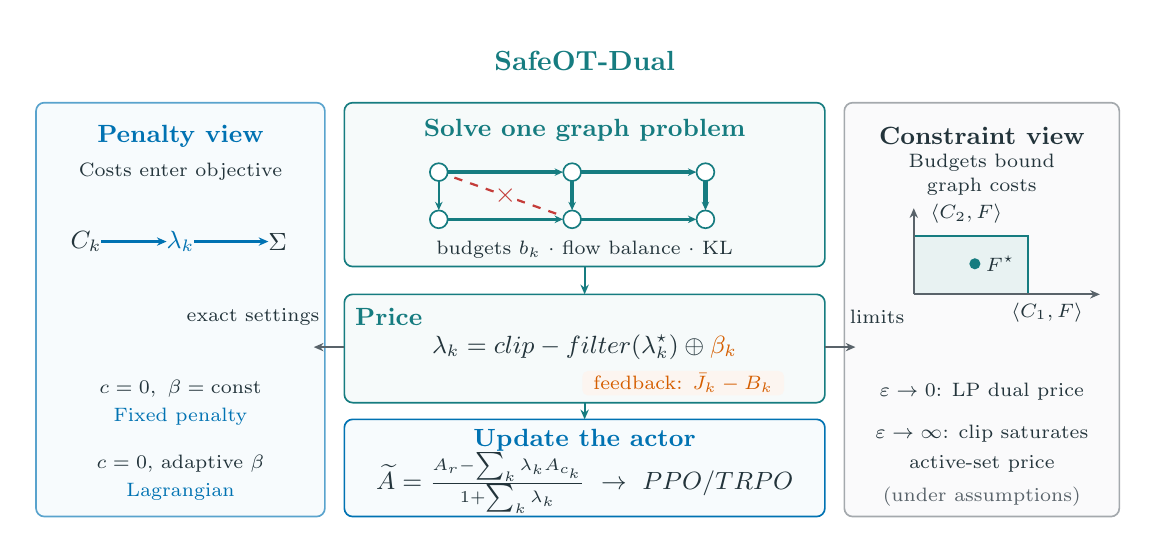
\begin{tikzpicture}[x=1bp,y=-1bp]

\path[use as bounding box] (0,0) rectangle (396,180);
% The three-column scaffold is fixed before any content is placed.
\draw[module,draw=blue!65,fill=blue!3] (3,27) rectangle (107,176);
\draw[module,draw=gray!55,fill=gray!3] (294,27) rectangle (393,176);
\draw[module,draw=teal,fill=teal!4] (114,27) rectangle (287,86);
\draw[module,draw=teal,fill=teal!4] (114,96) rectangle (287,135);
\draw[module,draw=blue,fill=blue!3] (114,141) rectangle (287,176);
\node[title,text=teal,font=\fontsize{10}{11}\selectfont\bfseries] at (200.5,12) {SafeOT-Dual};

% Left view: exact controller settings, not recovered external algorithms.
\node[title,text=blue] at (55,39) {Penalty view};
\node at (55,52) {Costs enter objective};
\node[formula] (cost) at (21,77) {$C_k$};
\node[formula,text=blue] (priceleft) at (55,77) {$\lambda_k$};
\node[formula] (sumleft) at (90,77) {$\Sigma$};
\draw[flow,blue] (cost.east) -- (priceleft.west);
\draw[flow,blue] (priceleft.east) -- (sumleft.west);
\node at (55,130) {$c=0,\ \beta=\mathrm{const}$};
\node[text=blue] at (55,140) {Fixed penalty};
\node at (55,157) {$c=0$, adaptive $\beta$};
\node[text=blue] at (55,167) {Lagrangian};

% Center: one constrained graph solve, one total price, one actor update.
\node[title,text=teal] at (200.5,37) {Solve one graph problem};
\foreach \name/\x/\y in {a/148/52,b/196/52,c/244/52,d/148/69,e/196/69,f/244/69}
  \coordinate (\name) at (\x,\y);
\draw[edge,teal,line width=1.7bp] (a) -- (b);
\draw[edge,teal,line width=1.7bp] (b) -- (c);
\draw[edge,teal,line width=.9bp] (a) -- (d);
\draw[edge,teal,line width=1.2bp] (b) -- (e);
\draw[edge,teal,line width=1.5bp] (c) -- (f);
\draw[edge,teal,line width=1.2bp] (d) -- (e);
\draw[edge,teal,line width=1.2bp] (e) -- (f);
\draw[line width=.8bp,dashed,hard] (a) -- (e);
\node[font=\fontsize{10}{10}\selectfont,text=hard,fill=teal!4,inner sep=.2bp] at (172,60.5) {$\times$};
\foreach \name in {a,b,c,d,e,f}
  \filldraw[fill=white,draw=teal,line width=.6bp] (\name) circle (3.2bp);
\node at (200.5,80) {budgets $b_k$ $\cdot$ flow balance $\cdot$ KL};
\draw[flow,teal] (200.5,86) -- (200.5,96);

\node[title,text=teal] at (130,104) {Price};
\node[formula] at (200.5,115) {$\lambda_k=\text{clip-filter}(\lambda_k^\star)\oplus {\color{orange}\beta_k}$};
\node[text=orange,fill=orange!6,rounded corners=2bp,inner xsep=4bp,inner ysep=1bp] at (236,128) {feedback: $\bar J_k-B_k$};
\draw[flow,teal] (200.5,135) -- (200.5,141);
\draw[flow,gray] (114,115) -- (103,115);
\node[anchor=east] at (105,104) {exact settings};
\draw[flow,gray] (287,115) -- (298,115);
\node[anchor=west] at (296,104) {limits};

\node[title,text=blue] at (200.5,148.5) {Update the actor};
\node[formula] at (200.5,164) {$\widetilde A=\frac{A_r-\sum_k\lambda_k A_{c_k}}{1+\sum_k\lambda_k}\ \to\ \text{PPO/TRPO}$};

% Right view: the shaded rectangle depicts only the two displayed budgets.
\node[title] at (343.5,39) {Constraint view};
\node[align=center] at (343.5,53) {Budgets bound\\graph costs};
\fill[teal!10] (319,75) rectangle (360,96);
\draw[line width=.6bp,teal] (319,75) -- (360,75) -- (360,96);
\draw[flow,gray] (319,96) -- (386,96);
\draw[flow,gray] (319,96) -- (319,65);
\node[anchor=west] at (325,67) {$\langle C_2,F\rangle$};
\node[anchor=north] at (367,99) {$\langle C_1,F\rangle$};
\fill[teal] (341,85) circle (2bp);
\node[anchor=west] at (345,85) {$F^\star$};
\node at (343.5,131) {$\varepsilon\to0$: LP dual price};
\node at (343.5,146) {$\varepsilon\to\infty$: clip saturates};
\node at (343.5,157) {active-set price};
\node[text=gray] at (343.5,169) {(under assumptions)};
\end{tikzpicture}
\end{document}
